\chapter{人工智能的基础与历史演进}
\label{chap:ai_basics}

\section{引言}
\label{sec:intro_chap1}
人工智能(Artificial Intelligence, AI)作为一门旨在研究、开发和应用能够模拟、延伸乃至超越人类智能的理论、方法、技术及应用系统的交叉学科,已成为引领新一轮科技革命和产业变革的核心驱动力。其研究领域不仅涵盖了从问题解决、知识推理到感知、学习和语言理解等传统智能行为的模拟,更拓展至自主决策、模式识别和创造性任务等前沿领域。本章旨在系统性地追溯人工智能的哲学起源与理论基础,阐述其核心概念体系,并深度剖析其在半个多世纪发展历程中的关键转折点、重大范式转移以及周期性的“寒冬”与复兴。通过对历史脉络的梳理,本章将为读者全面理解现代人工智能,特别是以深度学习为代表的技术浪潮,奠定坚实的理论与认知基础。

\section{核心概念与定义}
\label{sec:core_concepts}

\subsection{人工智能的定义}
\label{ssec:ai_definition}
人工智能的定义随着时代和技术发展而不断演变,至今未有完全统一的定论。一个广为接受的定义来自于Russell和Norvig的权威著作《人工智能:一种现代方法》,该书从思想和行为两个维度,以及与人类和理性的对比,将AI的定义分为了四个流派:
\begin{itemize}
    \item \textbf{像人一样思考(Thinking Humanly):} 这一流派致力于通过认知建模来模拟人类的思维过程。其核心是探究人类心智的内在机制,并用计算机程序来复现。
    \item \textbf{像人一样行动(Acting Humanly):} 该流派关注系统外部行为的表现,以著名的“图灵测试”为代表,即如果机器的行为表现与人类无法区分,则可认为其具备智能。
    \item \textbf{理性地思考(Thinking Rationally):} 该流派追求构建基于逻辑法则的推理系统。它根植于数理逻辑,旨在通过形式化推理得出正确结论,其代表是“逻辑主义”方法。
    \item \textbf{理性地行动(Acting Rationally):} 该流派关注于构建能够实现最优结果的“智能体”(Agent)。一个理性的智能体应在给定信息和环境下,采取能最大化其期望效用的行动。
\end{itemize}

一个理性的智能体在选择行动时,会遵循期望效用最大化原则。若智能体当前处于状态 $s$,可选择的行动集合为 $A$,采取行动 $a \in A$ 后可能转移到新状态 $s'$ 的概率为 $P(s'|s, a)$,且新状态的效用为 $U(s')$,则最优行动 $a^*$ 的选择可以表示为:
$$ a^* = \arg\max_{a \in A} \sum_{s'} P(s' |s, a) U(s') $$
这个公式定义了理性智能体如何在不确定的结果中做出最优决策。

在当前的工程实践和学术研究中,\textbf{理性地行动}已成为主流范式。它不仅包含了逻辑推理,也容纳了在不确定性下做出最优决策的能力,更具普适性和可度量性。

\subsection{强人工智能与弱人工智能}
\label{ssec:strong_weak_ai}
在人工智能理论中,根据其智能水平和通用性,通常将AI分为强人工智能和弱人工智能:

\begin{figure}[H]
    \centering
    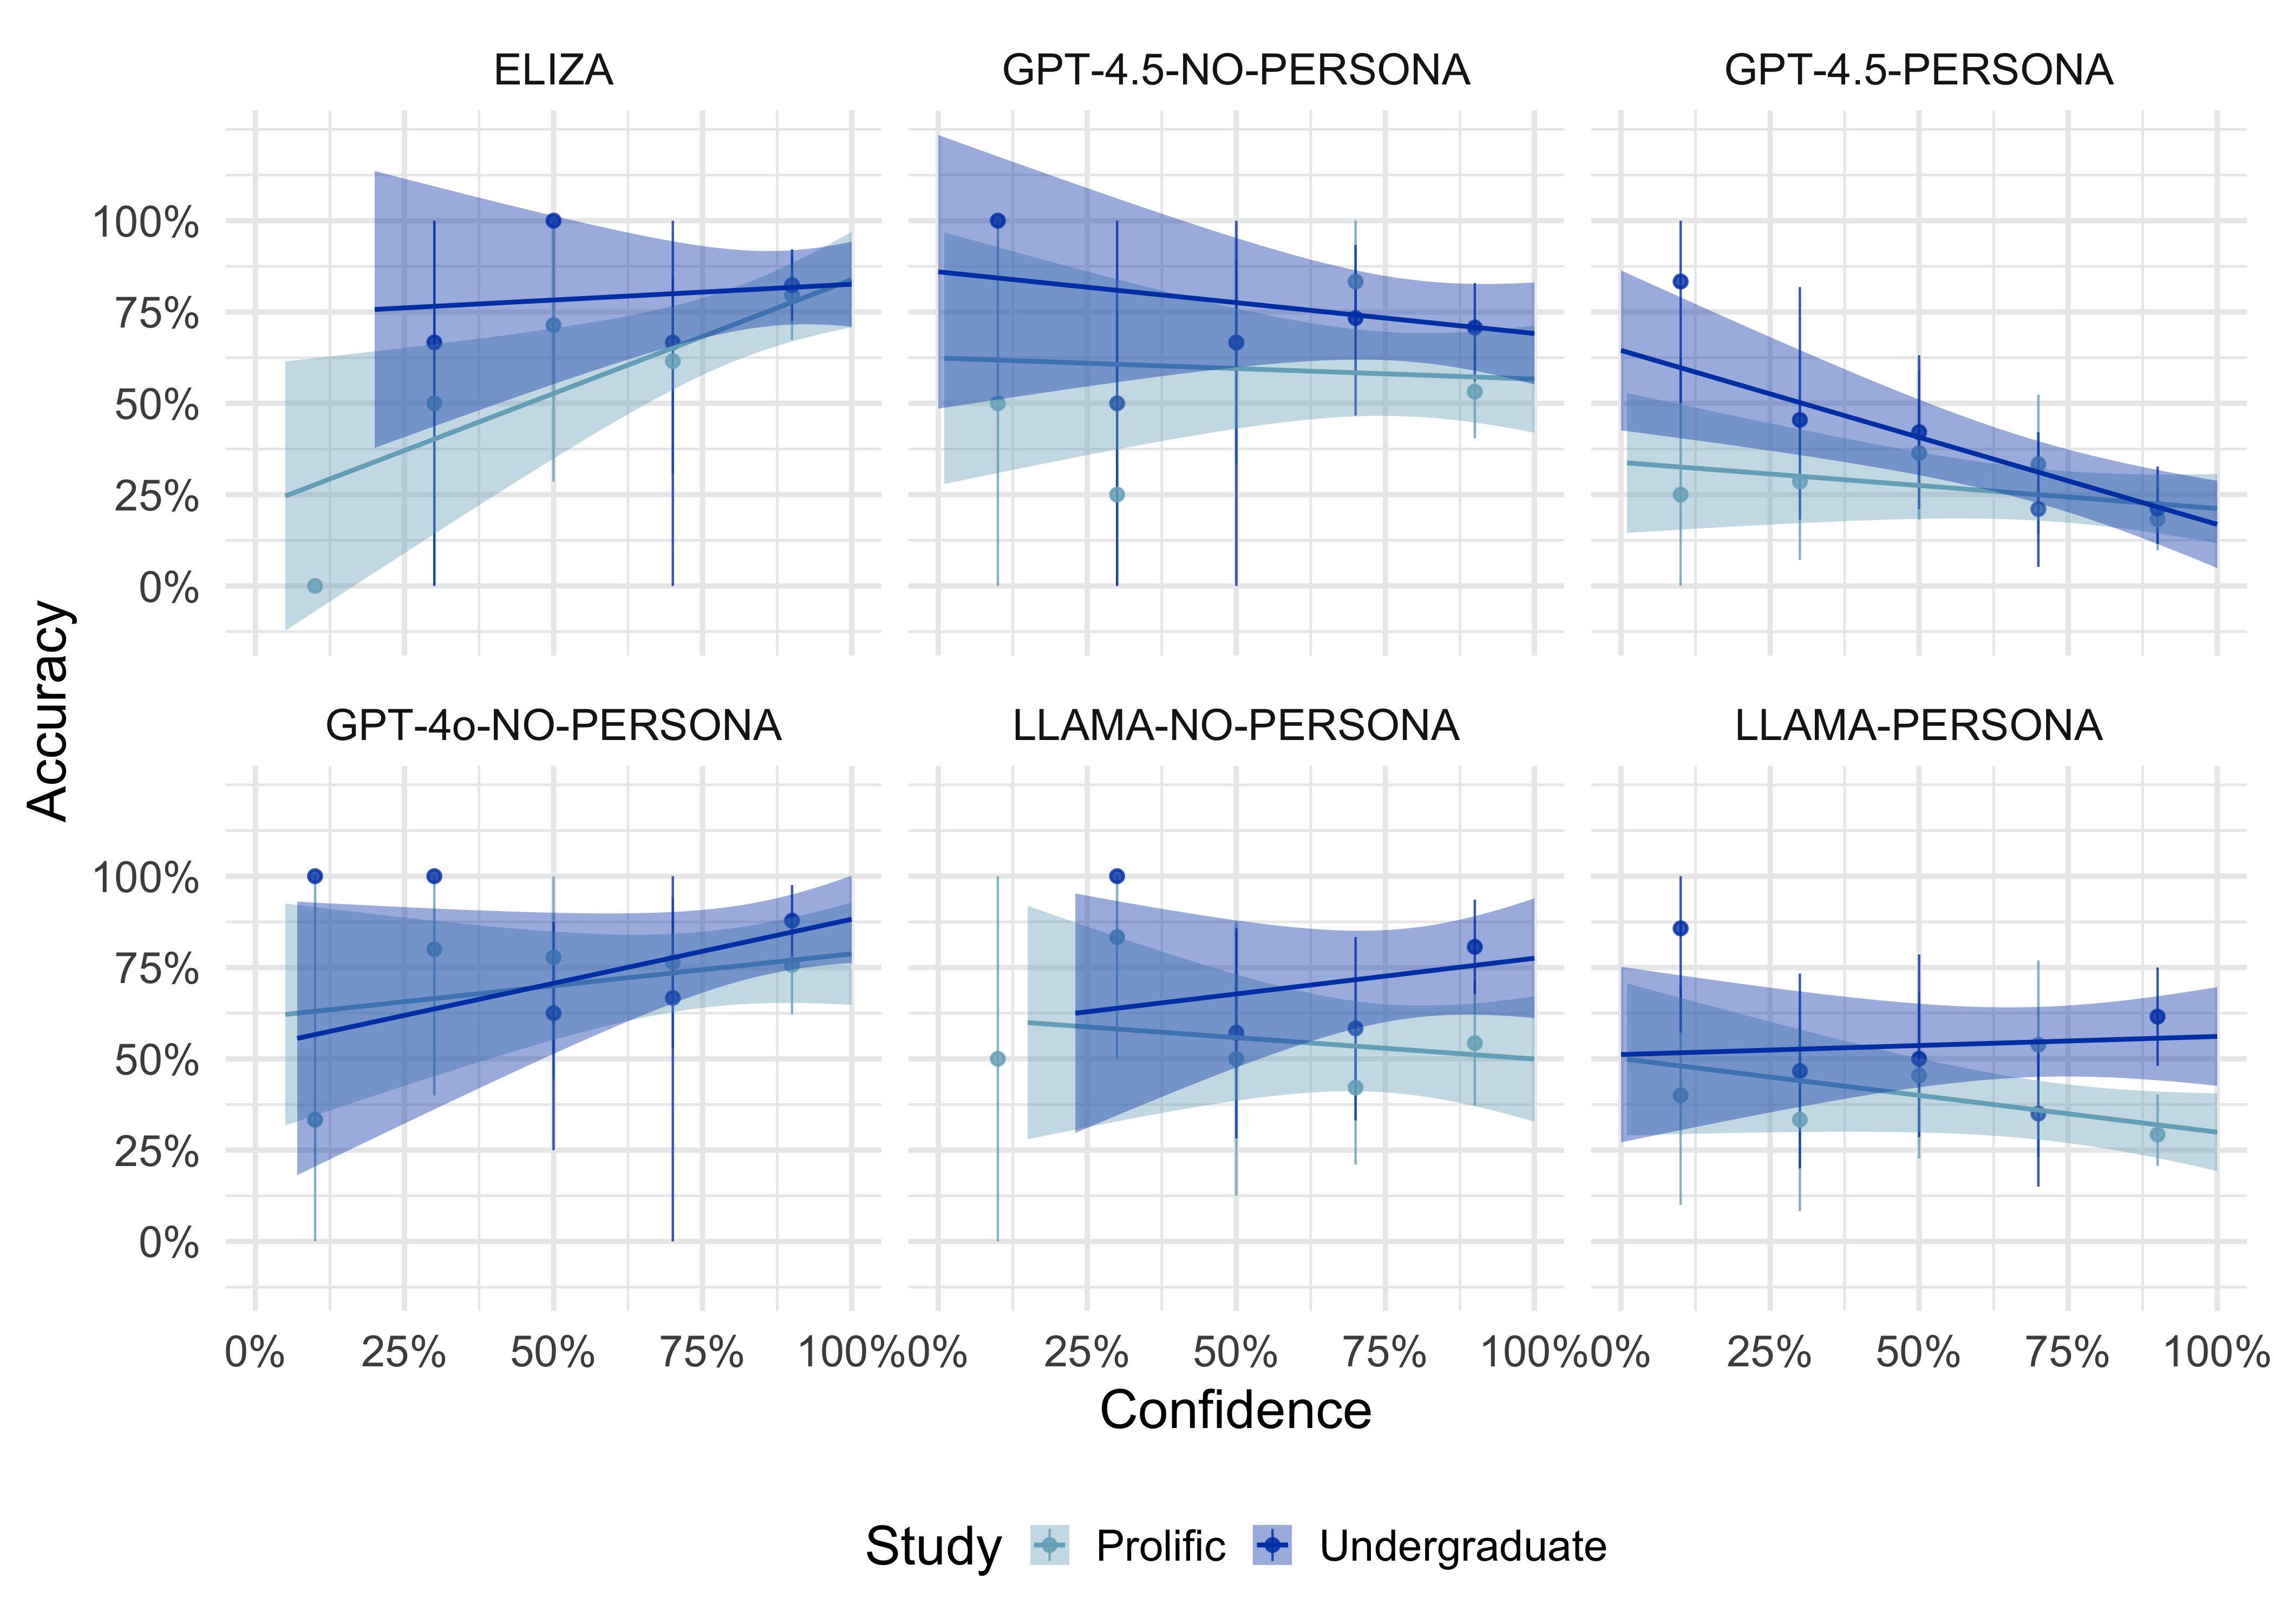
\includegraphics[width=0.8\textwidth]{contray.png} 
    \caption{强人工智能与弱人工智能的区别示意图}
    \label{fig:contray}
\end{figure}

\begin{itemize}
    \item \textbf{弱人工智能(Weak AI / Narrow AI):} 指的是专注于执行单一或有限领域特定任务的AI系统。例如,AlphaGo虽然在围棋上超越了人类顶尖棋手,但它无法执行如驾驶汽车或诊断疾病等其他任务。当前我们所看到并广泛应用的AI技术,如语音助手、推荐系统和人脸识别,绝大多数都属于弱人工智能范畴。
    \item \textbf{强人工智能(Strong AI / Artificial General Intelligence, AGI):} 指的是拥有与人类智能相当甚至超越人类智能的通用AI系统。理论上,一个AGI系统能够理解、学习并执行任何人类能够完成的智力任务,并具备自我意识、情感和抽象思维能力。强人工智能是AI研究的终极目标之一,但目前在理论和技术上仍面临巨大挑战,处于理论探索阶段。
\end{itemize}

\subsection{机器学习与深度学习概述}
\label{ssec:ml_dl_overview}
\textbf{机器学习(Machine Learning, ML)}\cite{mahesh2020machine}是实现人工智能的核心途径,其本质是让计算机通过分析数据来自动学习和改进,而非依赖于人类编写的显式规则。其核心思想是构建一个数学模型,该模型能够从训练数据中学习到潜在的模式或规律,并利用这些规律对新的、未知的数据进行预测或决策。根据学习方式的不同,机器学习主要分为以下几类:

\begin{figure}[H]
    \centering
    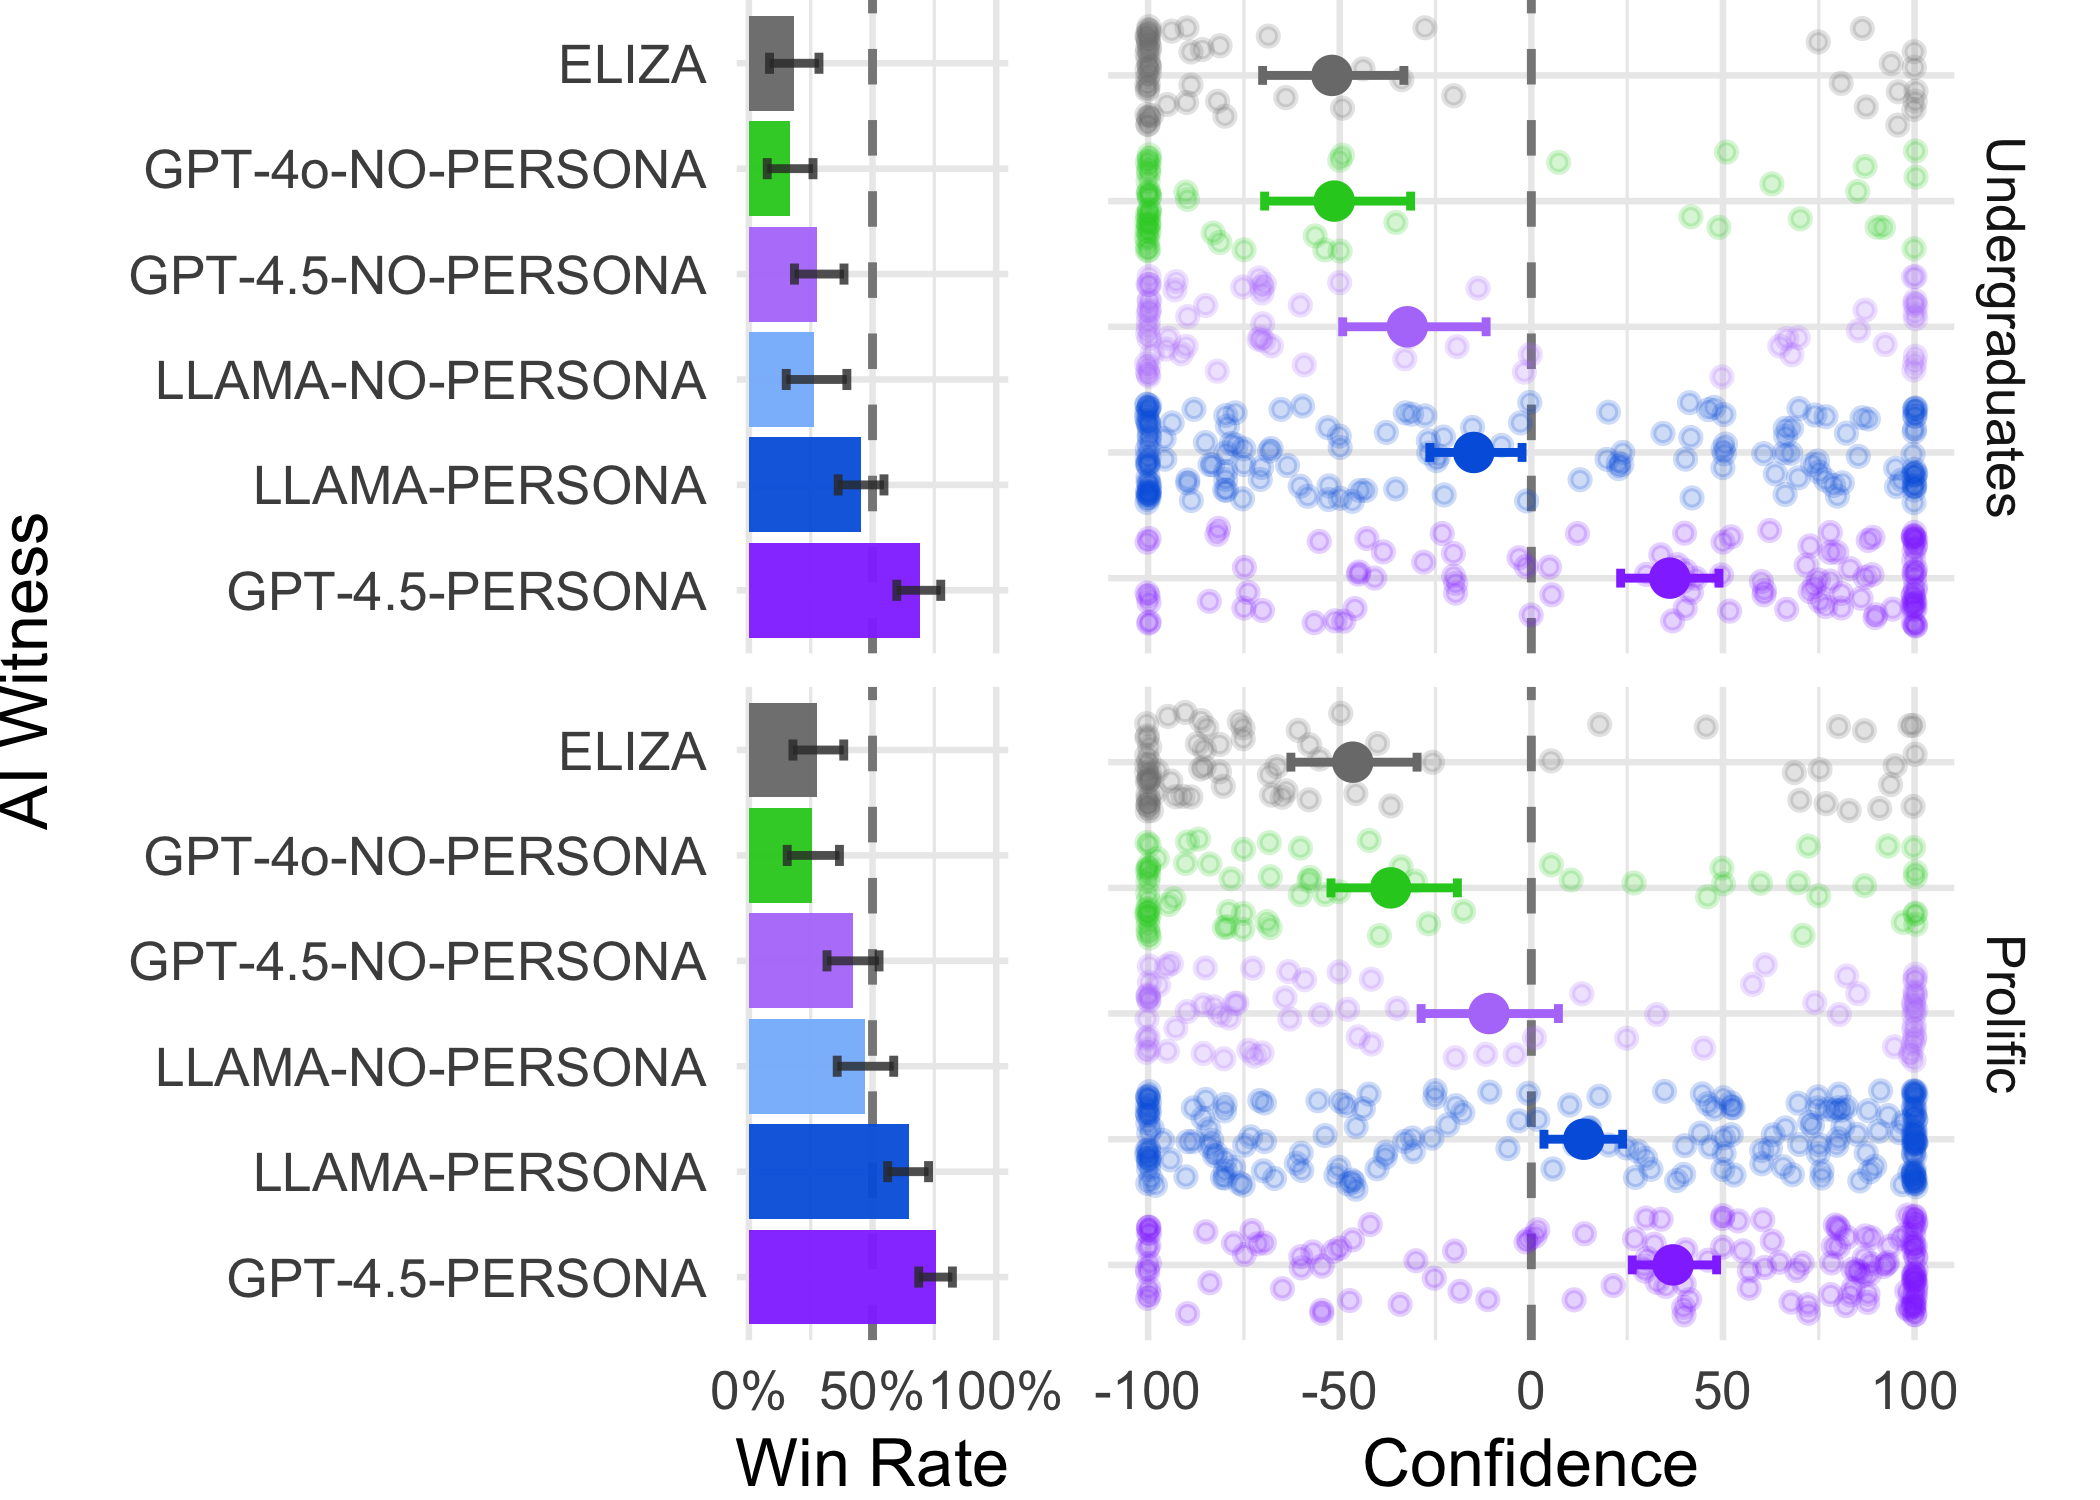
\includegraphics[width=0.8\textwidth]{rate.png} 
    \caption{机器学习的主要类型示意图}
    \label{fig:rate}
\end{figure}

\begin{itemize}
    \item \textbf{监督学习(Supervised Learning):}\cite{lecun2015deep} 模型从带有“正确答案”(即标签)的数据中学习。例如,在图像分类任务中,模型学习大量已标记为“猫”或“狗”的图片,最终学会识别新的图片。在数学上,给定一个包含 $N$ 个样本的训练数据集 $D = \{(x_1, y_1), (x_2, y_2), \dots, (x_N, y_N)\}$,其中 $x_i$ 是输入特征,$y_i$ 是对应的标签。监督学习的目标是学习一个从输入到输出的映射函数 $h_{\theta}$,该函数由参数 $\theta$ 决定,旨在最小化一个损失函数 $L$,即:
    $$ \theta^* = \arg\min_{\theta} \frac{1}{N} \sum_{i=1}^{N} L(h_{\theta}(x_i), y_i) $$
  其中 $L$ 用来度量预测值 $h_{\theta}(x_i)$ 和真实值 $y_i$ 之间的差异。
    \item \textbf{无监督学习(Unsupervised Learning):}\cite{glielmo2021unsupervised} 模型处理没有标签的数据,并尝试发现数据内部的结构或模式。例如,在市场分析中,无监督学习可用于自动将客户划分为不同的群体。
    \item \textbf{强化学习(Reinforcement Learning):}\cite{matsuo2022deep} 模型通过与环境的交互来学习。智能体(Agent)在环境中采取行动,并根据行动结果获得奖励或惩罚,其目标是学习一个能最大化长期累积奖励的策略。AlphaGo的成功就是强化学习的经典案例。
    在强化学习中,智能体的目标是学习一个策略(policy)$\pi$,该策略指导智能体在每个状态 $s_t$ 选择能最大化未来累积奖励的行动 $a_t$。在时间步 $t$ 的未来折扣累积奖励(或称为“回报” $G_t$)定义为:
    $$ G_t = R_{t+1} + \gamma R_{t+2} + \gamma^2 R_{t+3} + \dots = \sum_{k=0}^{\infty} \gamma^k R_{t+k+1} $$
    其中 $R_{t+k+1}$ 是在未来第 $k$ 步获得的奖励,$\gamma \in [0, 1]$ 是折扣因子,用于平衡即时奖励和未来奖励的重要性。智能体的最终目标是找到最优策略 $\pi^*$,以最大化该回报的期望值。
\end{itemize}

\begin{figure}[H]
    \centering
    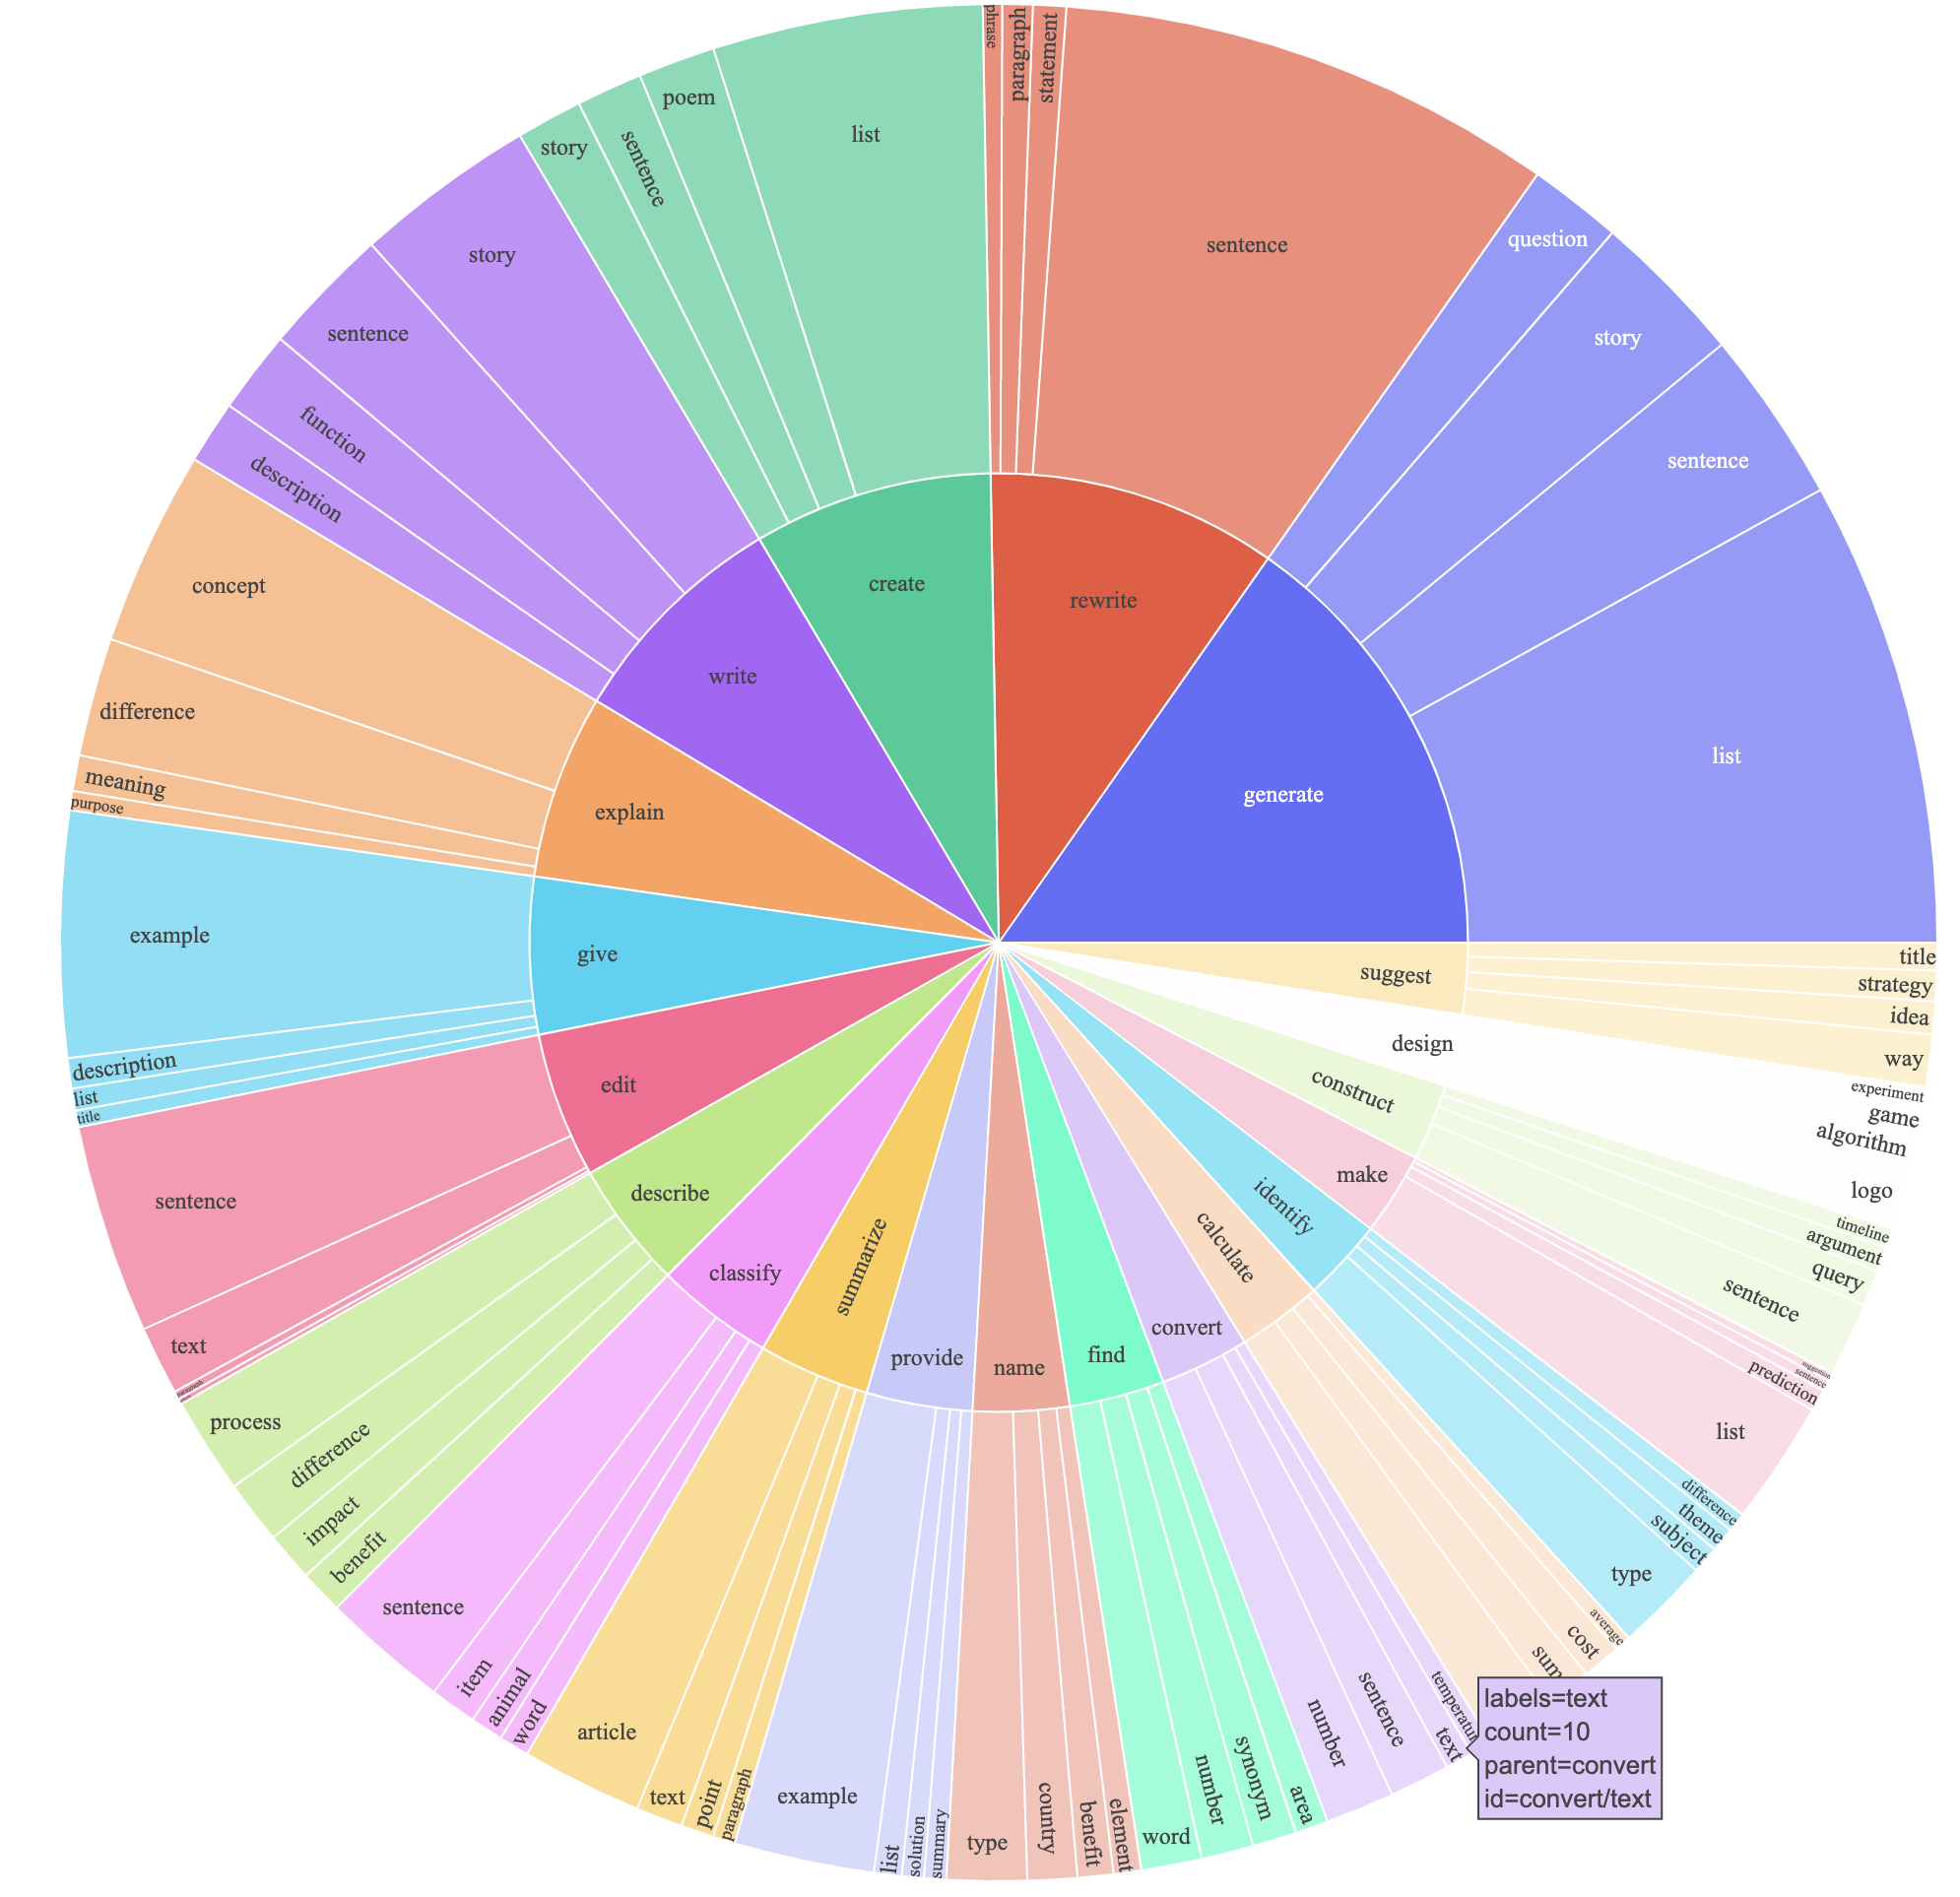
\includegraphics[width=0.8\textwidth]{parse.png} 
    \caption{机器学习的主要类型示意图}
    \label{fig:parse}
\end{figure}

\textbf{深度学习(Deep Learning, DL)}\cite{ahmed2023deep}是机器学习的一个强大分支,其核心是使用深度人工神经网络(Deep Neural Networks, DNNs)。“深度”通常指神经网络包含多个隐藏层。这种多层结构赋予了模型强大的特征学习能力:网络中的每一层可以对前一层输出的特征进行组合,从而学习到从低级到高级的、层层递进的特征表示(Feature Hierarchy)。例如,在图像识别中,第一层可能学习到边缘和颜色等基本特征,中间层可能学习到眼睛、鼻子等组合特征,而更高层则能识别出整张人脸。正是这种自动学习复杂特征的能力,使深度学习在图像识别、语音识别和自然语言处理等领域取得了前所未有的突破性进展,成为推动当前AI发展的核心引擎。
一个包含 $L$ 层的深度神经网络可以被看作是一个复合函数。对于输入 $X$,其最终输出 $Y_{pred}$ 的计算过程可以表示为:
$$ Y_{pred} = f(X) = f_L(\dots f_2(f_1(X; \theta_1)); \dots; \theta_L) $$
其中,$f_l$ 代表第 $l$ 层的运算,通常由一个线性变换和一个非线性激活函数 $\sigma$ 组成,即 $f_l(z; \theta_l) = \sigma(W_l z + b_l)$,$\theta_l = \{W_l, b_l\}$ 是该层的权重和偏置参数。这种层级结构使得网络能够自动学习从简单到复杂的数据特征。


\begin{figure}[H]
    \centering
    \begin{subfigure}[b]{0.45\textwidth} % <-- 注意宽度可以适当减小
        \centering
        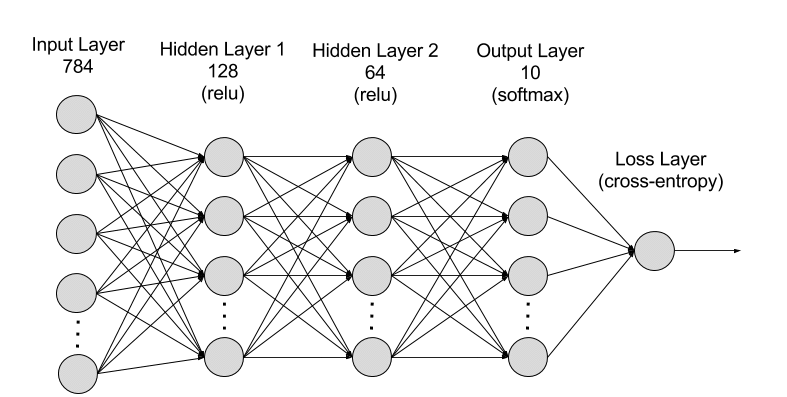
\includegraphics[height=4cm]{ai.png}
        \caption{人工智能、机器学习与深度学习的关系示意图}
        \label{fig:grouped_a}
    \end{subfigure}
    \hspace{1cm} 
    \begin{subfigure}[b]{0.45\textwidth}
        \centering
        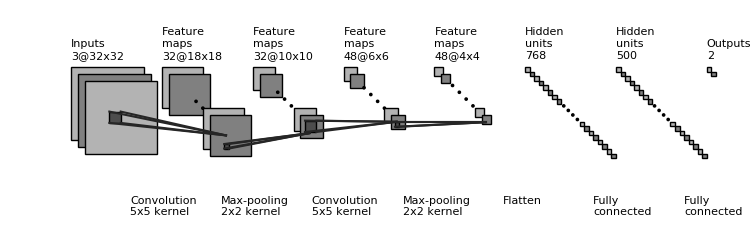
\includegraphics[height=4cm]{network.png}
        \caption{一个简单的神经网络结构示意图}
        \label{fig:grouped_b}
    \end{subfigure}
    \caption{人工智能、机器学习与深度学习的层级关系及神经网络结构}
    \label{fig:grouped_total}
\end{figure}

\section{哲学思辨与早期探索}
\label{sec:early_exploration}

\subsection{图灵测试与机器智能的界定}
\label{ssec:turing_test}
1950年,英国数学家、计算机科学的先驱阿兰·图灵(Alan Turing)在其划时代的论文《计算机器与智能》中,回避了“机器能否思考?”这一抽象的哲学问题,转而提出了一个可操作的“模仿游戏”,即后来的\textbf{图灵测试(Turing Test)}。该测试旨在通过一个行为主义的视角来检验机器是否能够展现出与人类无法区分的智能行为。在测试中,一位人类评审员通过纯文本界面同时与一位人类和一台机器进行交流。如果在持续的对话后,评审员无法可靠地分辨出哪个对话方是机器,那么这台机器就被认为通过了图灵测试。图灵测试为机器智能的评估提供了一个清晰、客观的操作性定义,虽然后续引发了诸多哲学上的争论(如“中文房间”思想实验),但其对早期人工智能研究的范式塑造和目标设定产生了深远影响。

\begin{figure}[H]
    \centering
    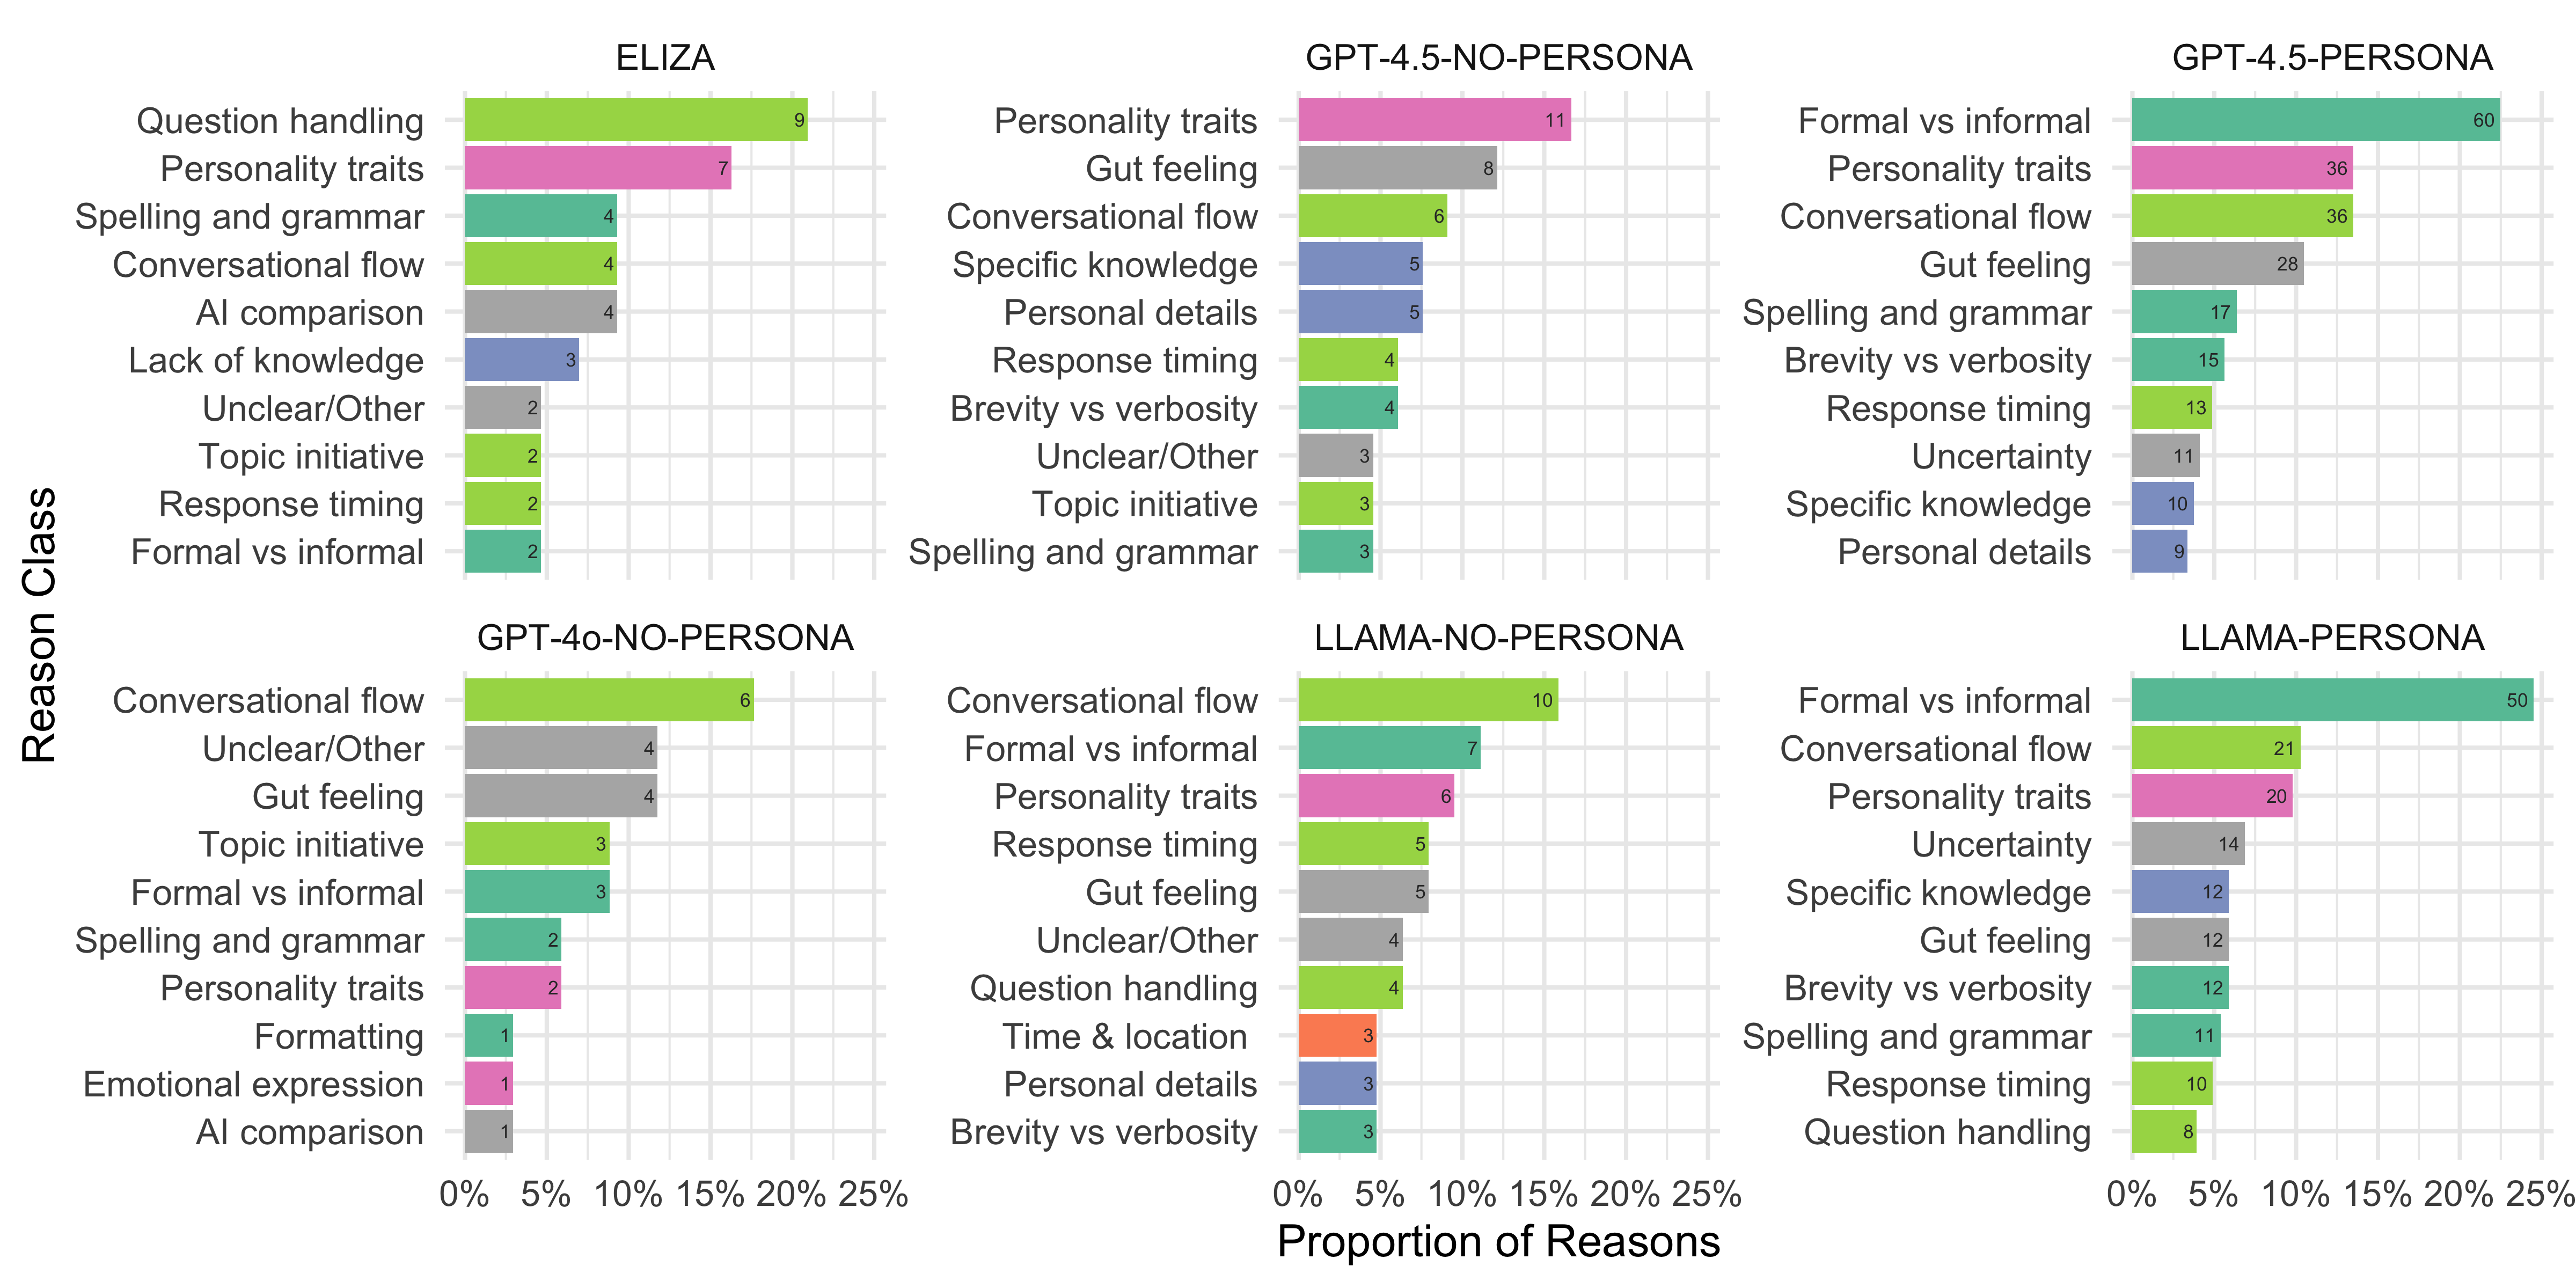
\includegraphics[width=0.8\textwidth]{Turing.png} 
    \caption{图灵测试示意图}
    \label{fig:turing_test}
\end{figure}

\subsection{达特茅斯会议与人工智能的诞生}
\label{ssec:dartmouth_conference}
1956年夏季,约翰·麦卡锡(John McCarthy)、马文·明斯基(Marvin Minsky)、克劳德·香农(Claude Shannon)和纳撒尼尔·罗切斯特(Nathaniel Rochester)等十位年轻学者在美国达特茅斯学院组织了一场为期两个月的学术研讨会。这次会议被普遍认为是“人工智能”这一学科正式诞生的标志。在为会议撰写的申请书中,麦卡锡首次创造了“Artificial Intelligence”一词。会议的目标宏大,旨在探索“学习的每个方面或智能的任何其他特征原则上都可以被精确描述,从而可以用机器来模拟它”。这次会议不仅确立了AI作为一个独立研究领域,还提出了许多至今仍被视为核心的基本问题,如自动推理、知识表示、自然语言处理和神经网络等,为未来数十年的研究议程奠定了基础。
\begin{figure}[H]
    \centering
    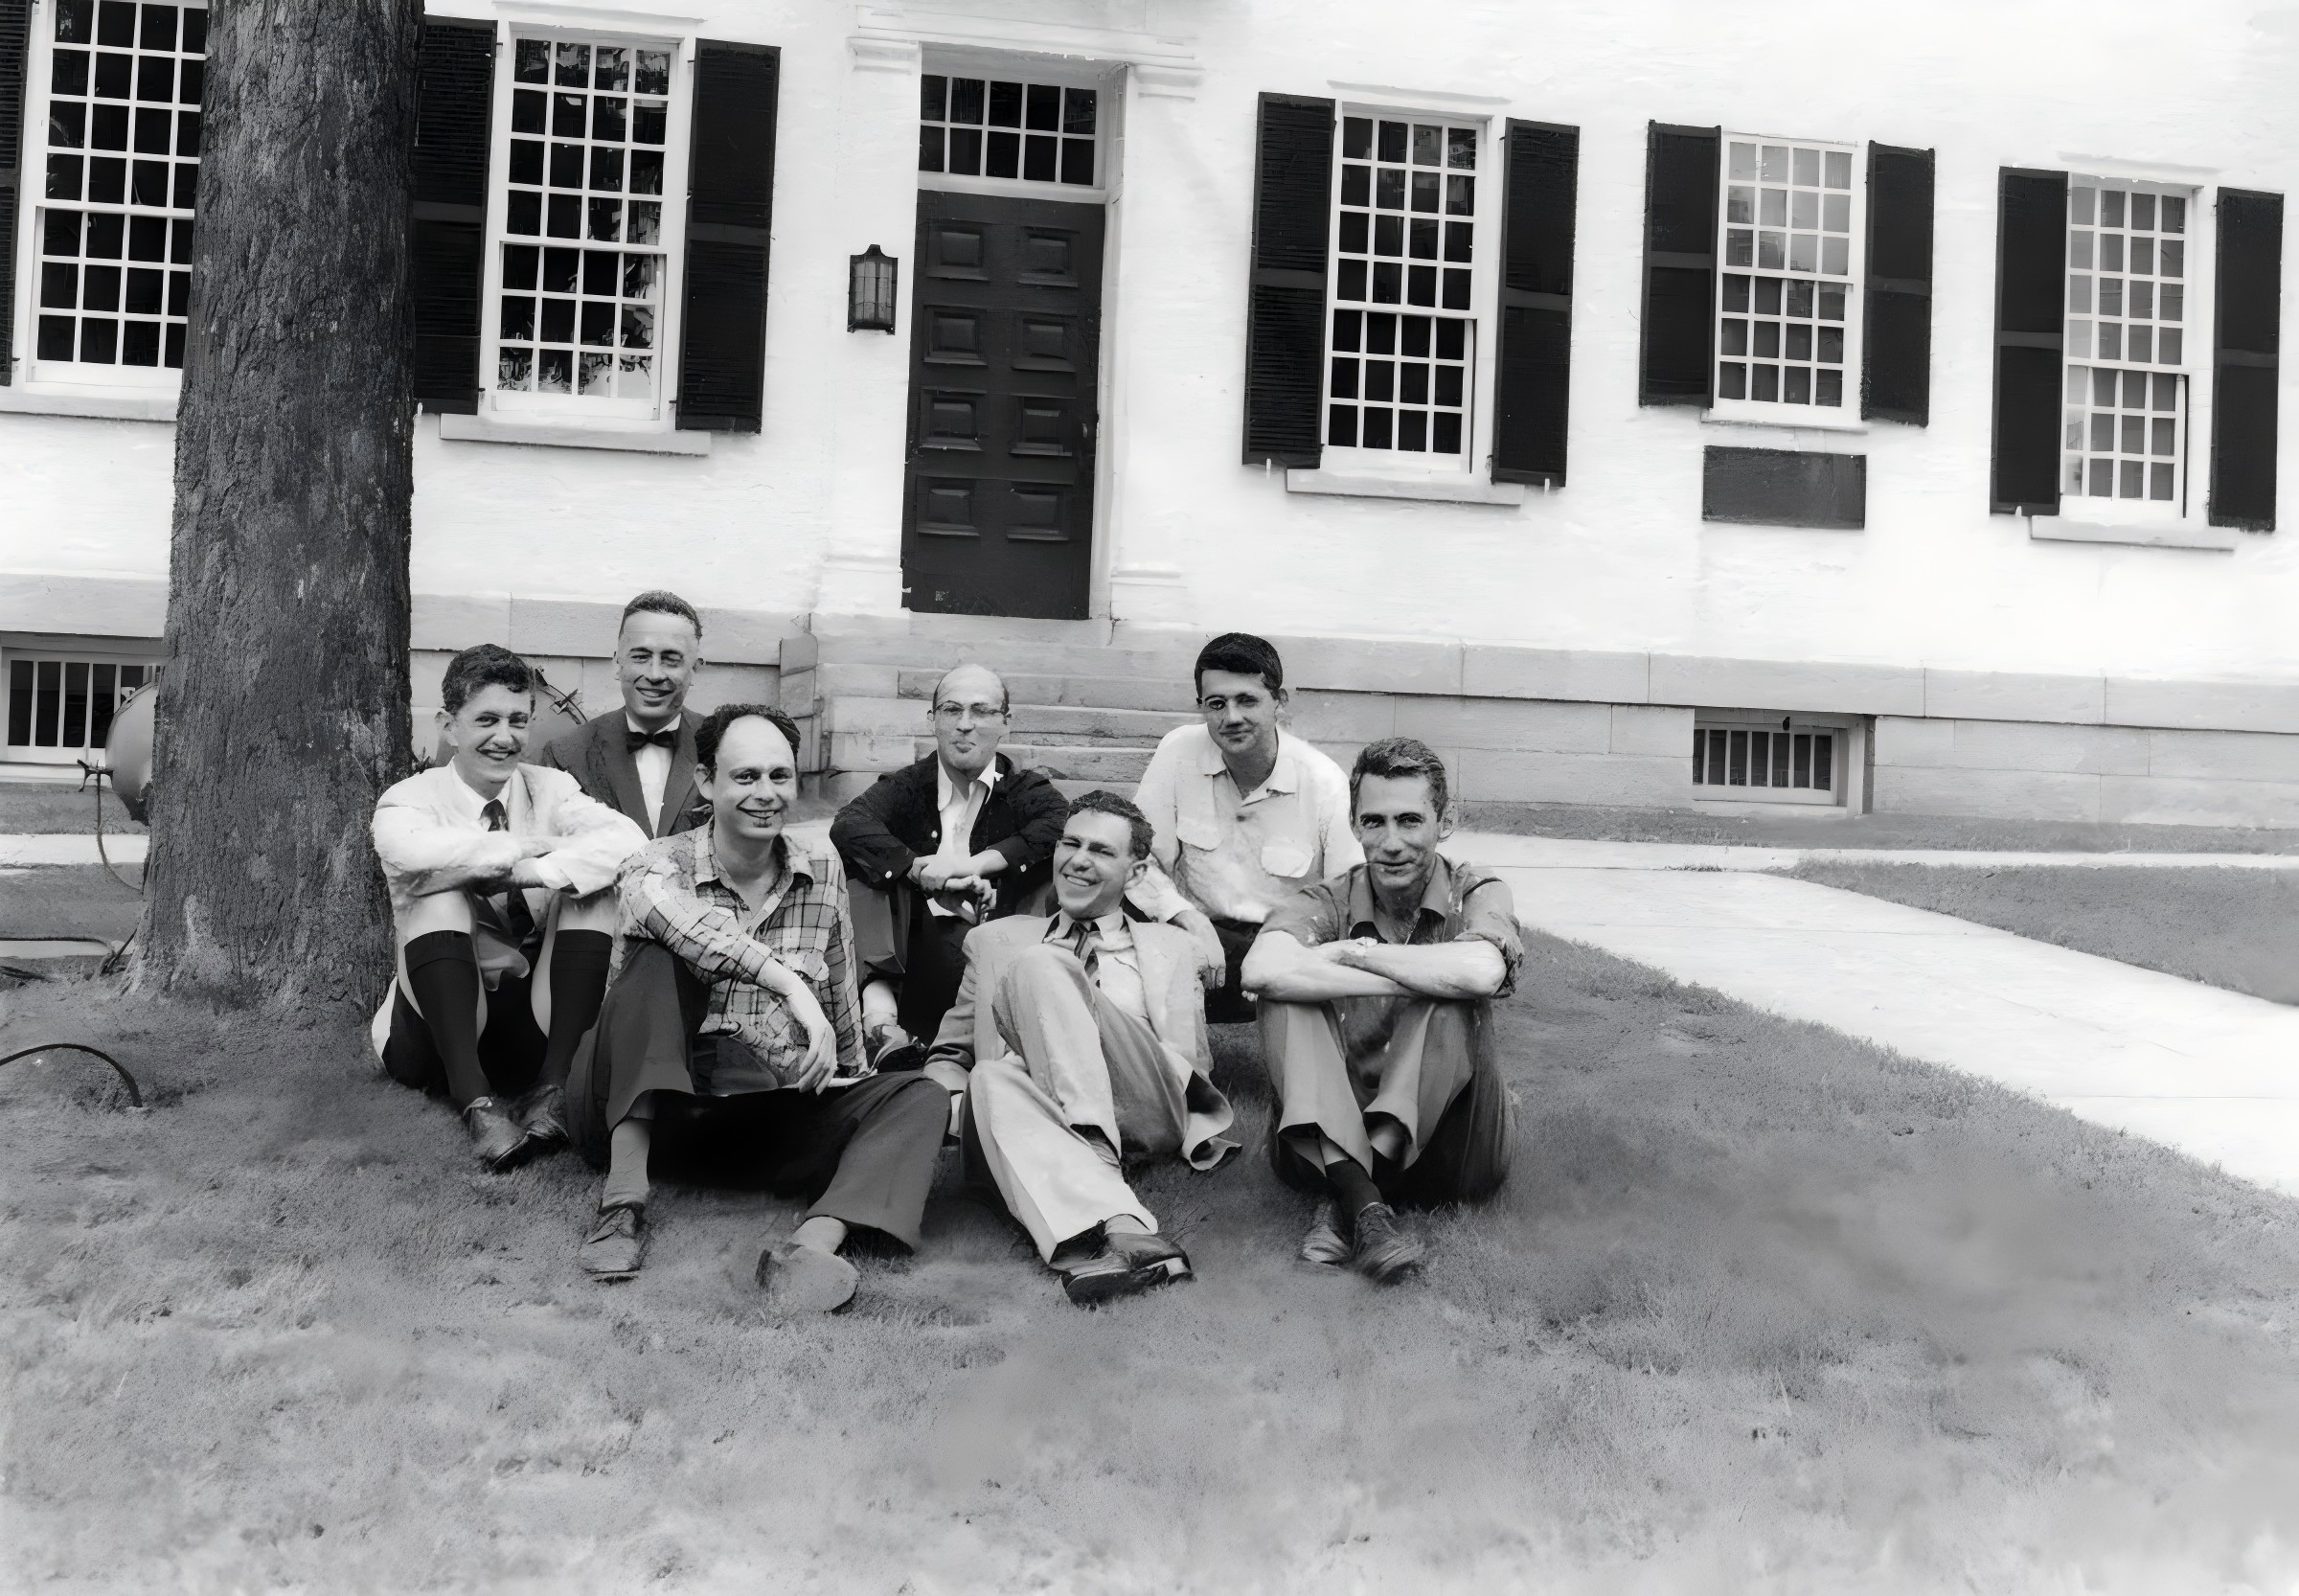
\includegraphics[width=0.8\textwidth]{dartmouth_conference.png} 
    \caption{达特茅斯会议的主要参与者}
    \label{fig:dartmouth_conference}
\end{figure}
\subsection{早期AI研究范式}
\label{ssec:early_paradigms}
达特茅斯会议之后,人工智能研究逐渐分化为两条主要的技术路线和哲学思想,即符号主义和连接主义。
\begin{itemize}
    \item \textbf{符号主义(Symbolism):}\cite{jung2023concerning} 也称逻辑主义或“整洁派”(Neats),其核心信念是:智能源于对符号的操作和逻辑推理。该范式认为,人类的认知过程本质上是一种符号处理过程,因此可以通过构建基于形式化逻辑和规则的系统来复现智能。这一思想主导了AI研究的前三十年,其代表性成果是专家系统(Expert Systems),例如在医学诊断(如MYCIN)和地质勘探等领域取得了显著的商业成功。然而,符号主义的“知识瓶颈”问题——即如何获取和编码海量、复杂的现实世界知识——最终限制了其发展。
    \item \textbf{连接主义(Connectionism):}\cite{maurer2021cognitive} 也称“邋遢派”(Scruffies),其灵感直接来源于生物大脑的神经网络结构。该范式认为,智能是从大量简单的、相互连接的处理单元(即人工神经元)的集体行为中“涌现”出来的,而非源于预设的符号规则。早期的感知机(Perceptron)是神经网络的基本组成单元,它接收多个输入信号 $x_i$,并通过一组权重 $w_i$ 进行加权求和,再加上一个偏置 $b$。其输出 $y$ 由一个阶跃函数(step function)决定:
    $$ y = f(\sum_{i=1}^{n} w_i x_i + b) \quad \text{其中} \quad f(z) = \begin{cases} 1 & \text{if } z > 0 \\ 0 & \text{otherwise} \end{cases} $$
    感知机模型为更复杂的神经网络奠定了基础。
    模型是连接主义的代表,但由于理论和计算能力的限制(特别是无法解决“异或”问题),连接主义在20世纪70年代后陷入了低谷,直到80年代中期反向传播算法的重新发现才得以复兴。
\end{itemize}
这两种范式在知识表示上存在根本差异:符号主义依赖于显式的、人类可理解的知识表达;而连接主义则通过网络连接的权重来隐式地学习和存储知识。

\section{AI的发展阶段与“寒冬”}
\label{sec:ai_stages_winters}

\subsection{第一次AI寒冬(约1974-1980年)}
\label{ssec:first_winter}
20世纪70年代中期,早期AI研究的乐观主义情绪遭遇了现实的严峻挑战。一方面,研究者在机器翻译等复杂任务上做出的过度承诺未能兑现;另一方面,面对组合爆炸问题,当时的计算能力和算法理论均显不足。标志性事件包括1966年美国自动语言处理咨询委员会(ALPAC)报告对机器翻译项目的悲观评估,以及1973年英国Lighthill报告对整个AI领域的严厉批评。这些事件直接导致了政府研究资助的大幅削减(尤其是美国的DARPA),研究者和资助机构的信心受到重创,AI领域进入了第一个被称为“寒冬”的低潮期。

\subsection{第二次AI寒冬(约1987-1993年)}
\label{ssec:second_winter}
在80年代,随着基于规则的专家系统(Expert Systems)\cite{shehadeh2024expert}的商业成功,AI迎来了一次短暂的复苏。然而,这些系统的局限性也逐渐暴露:它们的知识库构建和维护成本极其高昂、难以扩展、缺乏常识且无法处理不确定性。当企业发现维护这些专用系统的费用远超其带来的效益时,商业泡沫随之破裂。同时,个人电脑的兴起使得专门用于运行AI程序(如LISP语言)的昂贵硬件设备市场崩溃。这些因素共同导致了AI领域的第二次资金紧缩和信心危机,即第二次“AI寒冬”。

\subsection{AI的复兴与深度学习的爆发}
\label{ssec:ai_resurgence}
进入21世纪,特别是2010年以后,人工智能迎来了前所未有的复兴和爆发式增长。这并非偶然,而是由以下几个关键因素在“量变到质变”的临界点上协同作用的结果:
\begin{itemize}
    \item \textbf{海量数据(Big Data):} 互联网、移动设备和物联网的普及产生了前所未有的海量数据。像ImageNet这样包含超过1400万张手工标注图片的大规模数据集,为深度神经网络的训练提供了充足且高质量的“养料”,使其能够学习到过去无法企及的复杂模式。
    \item \textbf{硬件算力(Computing Power):} 摩尔定律的持续生效,特别是图形处理器(GPU)在通用计算领域的应用(GPGPU),为AI研究带来了革命性的变化。GPU高度并行的体系结构天然契合深度学习中的大规模矩阵和张量运算,使得过去需要数周甚至数月的训练时间缩短到几天或几小时,极大地加速了算法的迭代和优化。
    \item \textbf{核心算法(Algorithm Innovation):}\cite{xu2022separable} 深度学习算法本身也取得了关键性突破。2006年,Hinton等人提出的深度信念网络(DBN)和无监督预训练方法,有效解决了深度网络训练中的梯度消失问题。随后,诸如修正线性单元(ReLU)激活函数、Dropout正则化技术和批量归一化(Batch Normalization)等一系列创新,进一步简化和稳定了深度网络的训练过程。2012年,AlexNet模型在ImageNet图像识别挑战赛中以远超第二名的巨大优势夺冠,其成功标志着深度学习时代的正式开启。
\end{itemize}
这些因素形成了一个正向反馈循环:更强的算力支持更复杂的模型,更复杂的模型能从更大的数据集中学习,从而取得更好的效果,进而吸引更多的投入和研究,推动人工智能从实验室走向了广泛的工业和商业应用。

\section{总结}
\label{sec:conclusion_chap1}
本章系统性地回顾了人工智能从其哲学思辨的萌芽,到1956年达特茅斯会议上的正式诞生,历经两次因期望过高与现实局限而导致的“寒冬”,再到由数据、算力和算法共同驱动的深度学习复兴的完整历程。我们探讨了AI的四种核心定义范式,明确了强弱AI的本质区别,并阐明了机器学习与深度学习作为当前AI主流范式的层级关系与核心思想。早期符号主义与连接主义的对立与融合,为我们理解AI的不同技术路径提供了历史视角。

\begin{figure}[H]
    \centering
    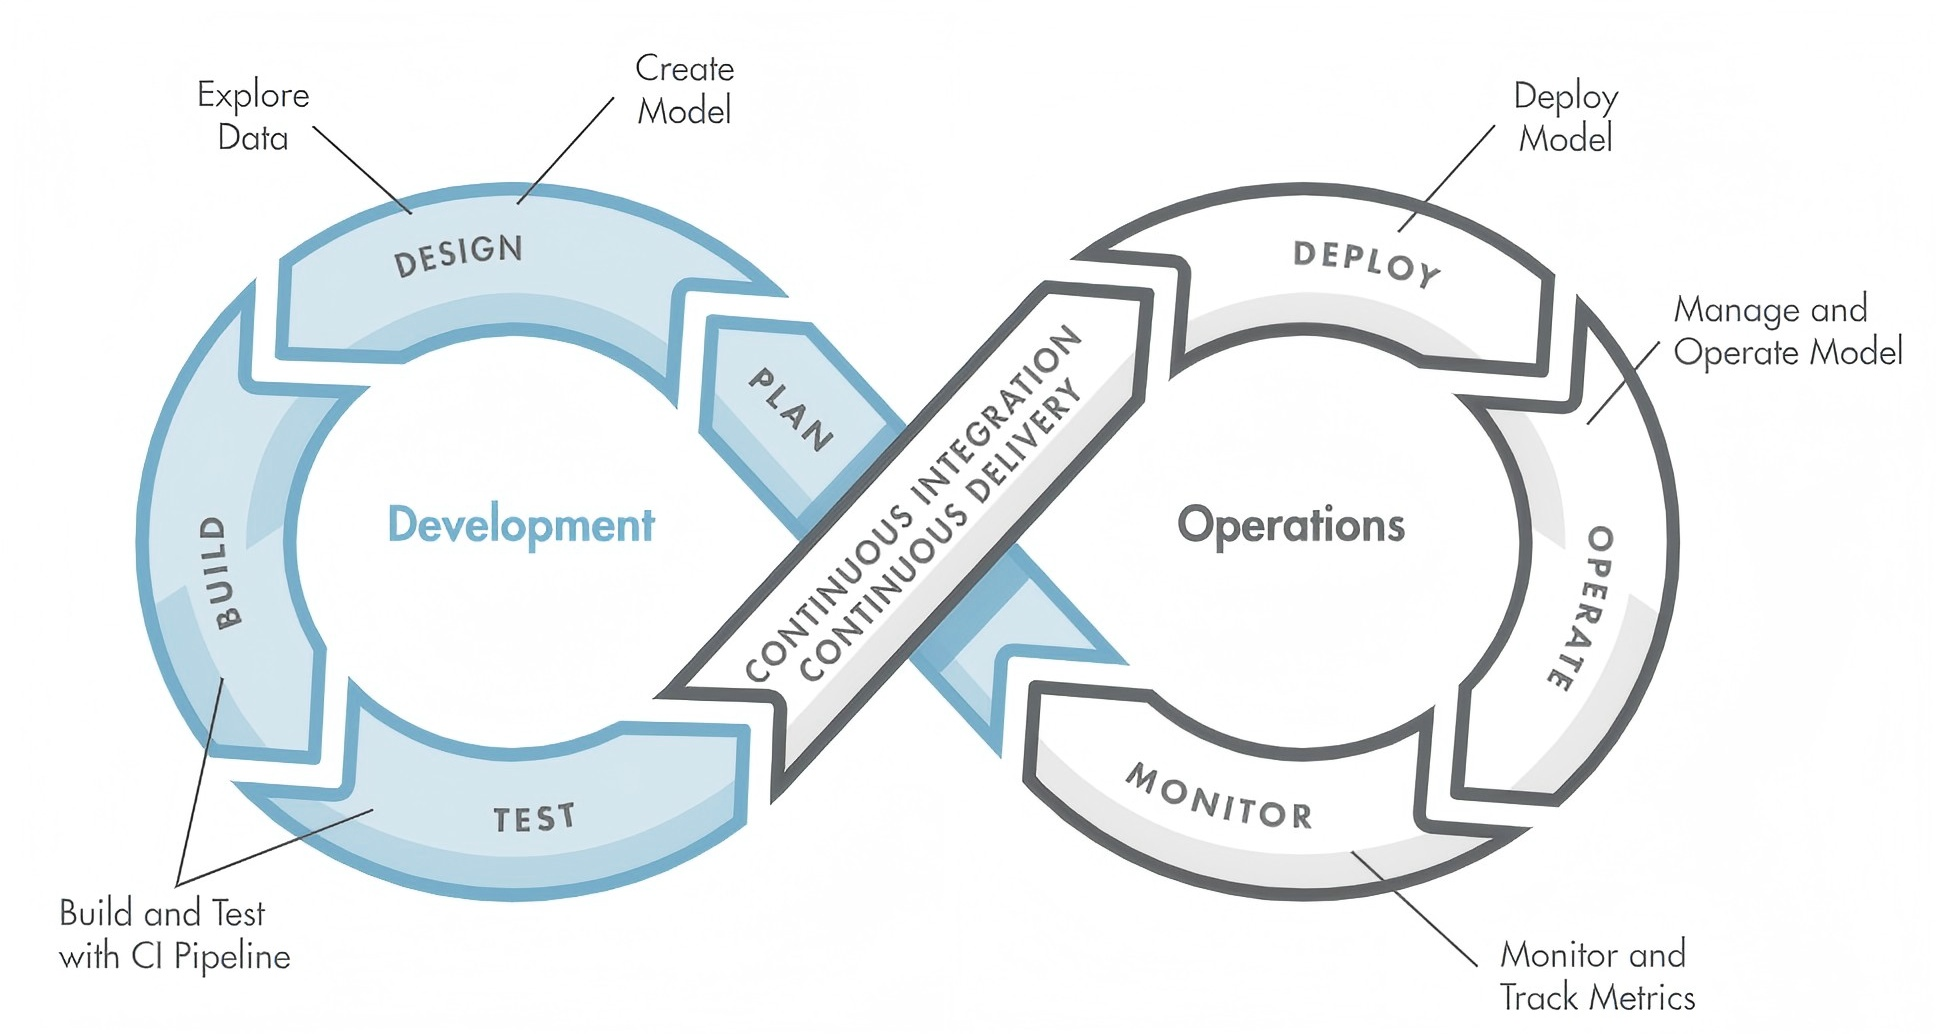
\includegraphics[width=0.8\textwidth]{circle.png} 
    \caption{人工智能发展历程的关键节点与范式演进}
    \label{fig:ai_history}
\end{figure}

\begin{figure}[H]
    \centering
    \begin{subfigure}[b]{0.48\textwidth}
        \centering
        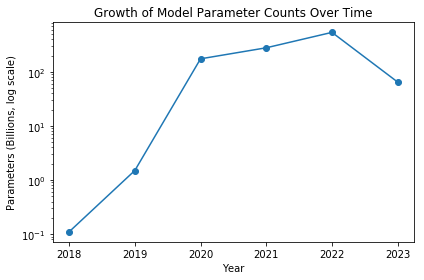
\includegraphics[width=\textwidth]{output1.png}
        \caption{模型参数量随时间增长情况}
        \label{fig:model_params_growth}
    \end{subfigure}
    \hfill 
    \begin{subfigure}[b]{0.48\textwidth}
        \centering
        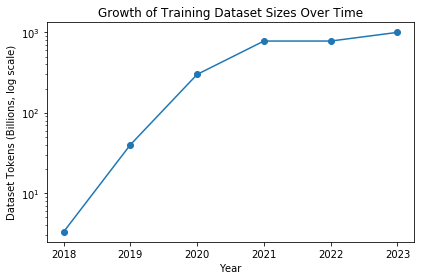
\includegraphics[width=\textwidth]{output2.png}
        \caption{训练数据集规模随时间增长情况}
        \label{fig:dataset_size_growth}
    \end{subfigure}
    
    \vspace{1cm} 
    
    \begin{subfigure}[b]{0.48\textwidth}
        \centering
        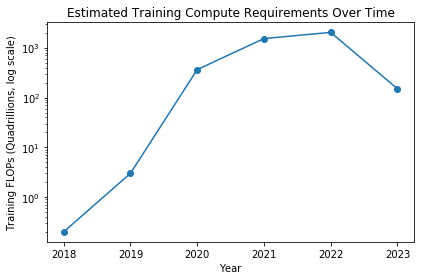
\includegraphics[width=\textwidth]{output3.png}
        \caption{训练所需算力随时间变化情况}
        \label{fig:compute_reqs_growth}
    \end{subfigure}
    \hfill 
    \begin{subfigure}[b]{0.48\textwidth}
        \centering
        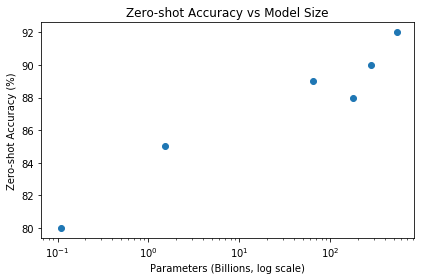
\includegraphics[width=\textwidth]{output4.png}
        \caption{模型零样本准确率与模型规模关系}
        \label{fig:accuracy_vs_size}
    \end{subfigure}

    \caption{驱动现代大型语言模型发展的关键要素量化趋势}
    \label{fig:llm_trends_overview}
\end{figure}